\documentclass[10pt]{article}
\usepackage[margin=1in]{geometry}
\usepackage{amsmath,amssymb,graphicx,hyperref,mathrsfs,siunitx}
\usepackage[small,bf]{caption}
\title{Isothermobaric Cr--Nb--Ni Phase Diagram}
\author{T. Keller}
\date{\small \today}

\frenchspacing
\hypersetup{linktocpage, colorlinks, citecolor=black, filecolor=black, linkcolor=black, urlcolor=blue}

\begin{document}
\maketitle

\section*{Assertion}

Nana Ofori-Opoku posited the following system of equations for each pair of phases $\alpha, \beta$
for a given test point with composition $(x_A, x_B)$:

\begin{align}
  \label{eqn:noo1}
  \frac{\partial f_{\alpha}}{\partial x_A^{\alpha}} -
  \frac{\partial f_{\beta}}{\partial x_A^{\beta}}
  &= 0\\
  \label{eqn:noo2}
  \frac{\partial f_{\alpha}}{\partial x_B^{\alpha}} -
  \frac{\partial f_{\beta}}{\partial x_B^{\beta}}
  &= 0\\
  \label{eqn:noo3}
  f_{\alpha}(x_A^{\alpha}, x_B^{\alpha}) +
  \frac{\partial f_{\alpha}}{\partial x_A^{\alpha}}\left(x_A^{\alpha} - x_A^{\beta}\right) +
  \frac{\partial f_{\alpha}}{\partial x_B^{\alpha}}\left(x_B^{\alpha} - x_B^{\beta}\right) -
  f_{\beta}(x_A^{\beta}, \partial x_B^{\beta})
  &= 0\\
  \label{eqn:noo4}
  \frac{x_A - x_A^{\beta}}{x_B - x_B^{\beta}} -
  \frac{x_A^{\alpha} - x_A^{\beta}}{x_B^{\alpha} - x_B^{\beta}}
  &= 0
\end{align}
This system can be solved numerically, and the result -- filtered to exclude phase-compositions
outside the Gibbs simplex -- is shown in Fig.~\ref{fig:noo-diagram}. The equations correspond to
\begin{enumerate}
    \item Equality of chemical potential of component $A$ in both phases.
    \item Equality of chemical potential of component $B$ in both phases.
    \item Equality of grand potentials in both phases, where
      \begin{equation}\label{eqn:gp}
        \Omega_{\psi} = f_{\psi}(x_A^{\psi}, x_B^{\psi}) +
                        \frac{\partial f_{\psi}}{\partial x_A^{\psi}}(x_A^{\psi}) +
                        \frac{\partial f_{\psi}}{\partial x_B^{\psi}}(x_B^{\psi})
      \end{equation}
    \item The lever rule for weight fractions, which can be derived from conservation of mass
          and the fact that the equilibrium volume fractions $\varphi^{\alpha} + \varphi^{\beta} = 1$.
      \begin{align}
        \label{eqn:consA}
        x_A &= x_A^{\alpha}\varphi^{\alpha} +
               x_A^{\beta} \varphi^{\beta} \\
        \label{eqn:consB}
        x_B &= x_B^{\alpha}\varphi^{\alpha} +
               x_B^{\beta} \varphi^{\beta} \\
        \label{eqn:lever}
        \frac{x_A - x_A^{\beta}}{x_A^{\alpha} - x_A^{\beta}} &=
        \frac{x_B - x_B^{\beta}}{x_B^{\alpha} - x_B^{\beta}}
      \end{align}
\end{enumerate}

\newpage
\begin{figure}[h]
  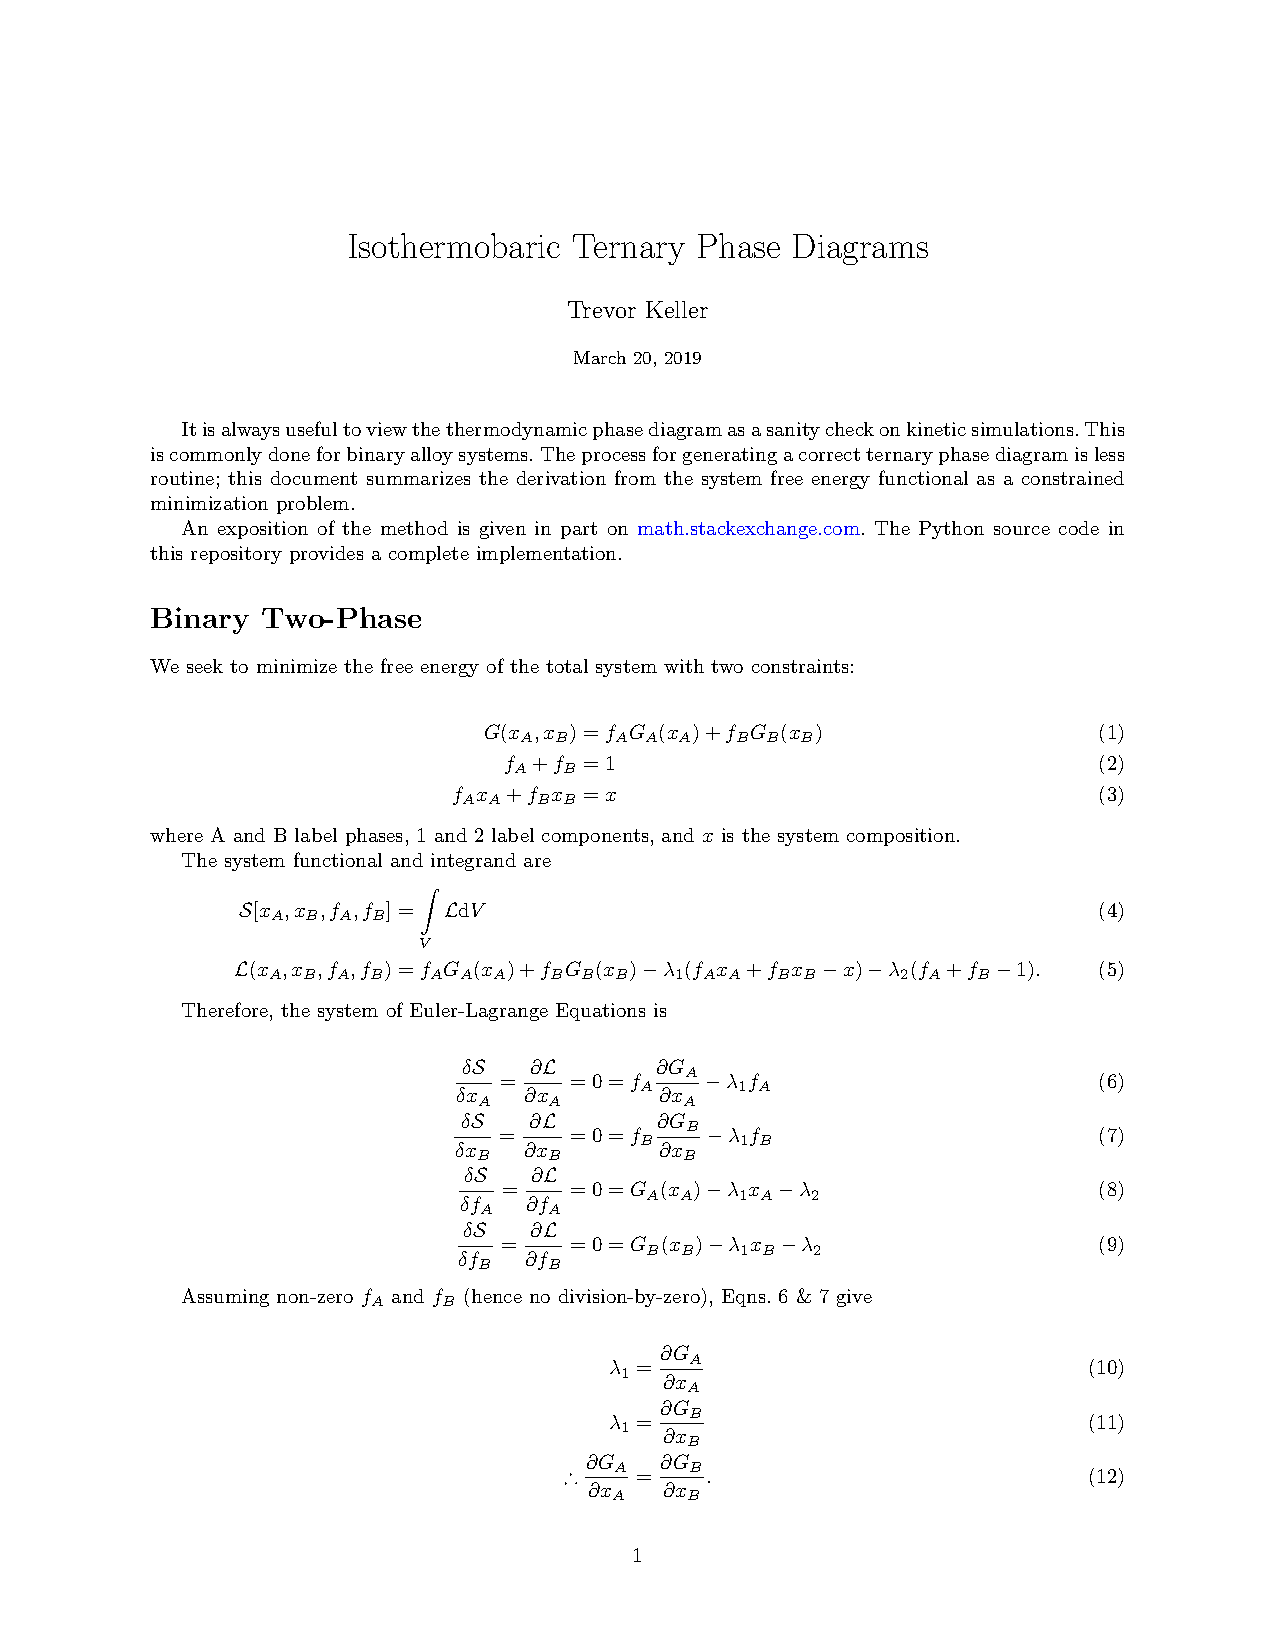
\includegraphics[width=\textwidth]{../ternary-diagram}
  \caption{Ternary diagram computed from Eqns.~\ref{eqn:noo1}--\ref{eqn:noo4}.
           Red spots correspond to endpoints of tie lines originating in $\gamma$ phase.
           Green spots correspond to endpoints of tie lines originating in $\delta$ phase.
           Blue spots correspond to endpoints of tie lines originating in Laves phase.
  }
  \label{fig:noo-diagram}
\end{figure}

\newpage
\section*{Derivation}

Jim Warren recommended a more fundamental approach, taking the system free energy
and applying mass conservation as constraints. An exposition of the method is given at
\href{https://math.stackexchange.com/questions/632/validating-a-mathematical-model-lagrange-formulation-and-geometry}
{math.stackexchange.com}.

\subsection*{Binary Two-Phase}

We seek to minimize the free energy of the total system with two constraints:

\begin{align}
  G(x_A, x_B) &= f_A G_A(x_A) + f_B G_B(x_B)\\
  f_A + f_B &= 1\\
  f_A x_A + f_B x_B &= x
\end{align}
where A and B label phases, 1 and 2 label components, and $x$ is the system composition.

The system functional and integrand are
\begin{align}
  \mathcal{S}[x_A, x_B, f_A, f_B] &= \int\limits_V\mathcal{L}\mathrm{d}V\\
  \mathcal{L}(x_A, x_B, f_A, f_B) &= f_A G_A(x_A) + f_B G_B(x_B) - \lambda_1(f_A x_A + f_B x_B - x) - \lambda_2(f_A + f_B - 1).
\end{align}

Therefore, the system of Euler-Lagrange Equations is

\begin{align}
  \label{eqn:el1}
  \frac{\delta\mathcal{S}}{\delta x_A} = \frac{\partial\mathcal{L}}{\partial x_A} = 0 &= f_A \frac{\partial G_A}{\partial x_A} - \lambda_1 f_A\\
  \label{eqn:el2}
  \frac{\delta\mathcal{S}}{\delta x_B} = \frac{\partial\mathcal{L}}{\partial x_B} = 0 &= f_B \frac{\partial G_B}{\partial x_B} - \lambda_1 f_B\\
  \label{eqn:el3}
  \frac{\delta\mathcal{S}}{\delta f_A} = \frac{\partial\mathcal{L}}{\partial f_A} = 0 &= G_A(x_A) - \lambda_1x_A - \lambda_2\\
  \label{eqn:el4}
  \frac{\delta\mathcal{S}}{\delta f_B} = \frac{\partial\mathcal{L}}{\partial f_B} = 0 &= G_B(x_B) - \lambda_1x_B - \lambda_2
\end{align}

Assuming non-zero $f_A$ and $f_B$ (hence no division-by-zero), Eqns.~\ref{eqn:el1}~\&~\ref{eqn:el2} give

\begin{align}
  \lambda_1 &= \frac{\partial G_A}{\partial x_A}\\
  \lambda_1 &= \frac{\partial G_B}{\partial x_B}\\
  \label{eqn:chempot}
  \therefore \frac{\partial G_A}{\partial x_A} &= \frac{\partial G_B}{\partial x_B}.
\end{align}

Subtracting Eqns.~\ref{eqn:el3}$-$\ref{eqn:el4} gives
\begin{align}
  G_A(x_A) - G_B(x_B) &= \lambda_1(x_A - x_B)\\
  \label{eqn:grandpot}
  \therefore G_B(x_B) &= G_A(x_A) - \frac{\partial G_A}{\partial x_A}\left(x_A - x_B\right).
\end{align}

Eqn.~\ref{eqn:chempot} represents equality of chemical potential, while
Eqn.~\ref{eqn:grandpot} represents equality of grand potential energy. This pair
of equations can be solved to determine the two unknown compositions needed to
specify the equilibrium tie line containing points $G_A(x_A)$, $G(x)$, and
$G_B(x_B)$. These are similar to Nana's derivation, but in a reduced system.

\subsection*{Ternary Two-Phase}

We seek to minimize the free energy of the total system with three constraints:

\begin{align}
  G(x_1^A, x_2^A, x_1^B, x_2^B) &= f_A G_A(x_1^A,x_2^A) + f_B G_B(x_1^B, x_2^B)\\
  f_A x_1^A + f_B x_1^B &= x_1\\
  f_A x_2^A + f_B x_2^B &= x_2\\
  f_A + f_B &= 1
\end{align}
where A and B label phases, 1 and 2 label components, $x_1$ and $x_2$ are the system compositions,
and compositions with labels $x_i^j$ represent the composition of component $i$ in phase $j$.

The integrand is

\begin{align}
  \nonumber
  \mathcal{L}(x_1^A, x_2^A, x_1^B, x_2^B) &= f_A G_A(x_1^A, x_2^A) + f_B G_B(x_1^B, x_2^B)\\
  \nonumber
                                          &- \lambda_1(f_A x_1^A + f_B x_1^B - x_1)\\
  \nonumber
                                          &- \lambda_2(f_A x_2^A + f_B x_2^B - x_2)\\
                                          &- \lambda_3(f_A + f_B - 1)
\end{align}

The system of Euler-Lagrange Equations becomes

\begin{align}
  \label{eqn:2el1}
  \frac{\partial\mathcal{L}}{\partial x_1^A} = 0 &= f_A \frac{\partial G_A}{\partial x_1^A} - \lambda_1 f_A\\
  \label{eqn:2el2}
  \frac{\partial\mathcal{L}}{\partial x_1^B} = 0 &= f_B \frac{\partial G_B}{\partial x_1^B} - \lambda_1 f_B\\
  \label{eqn:2el3}
  \frac{\partial\mathcal{L}}{\partial x_2^A} = 0 &= f_A \frac{\partial G_A}{\partial x_2^A} - \lambda_2 f_A\\
  \label{eqn:2el4}
  \frac{\partial\mathcal{L}}{\partial x_2^B} = 0 &= f_B \frac{\partial G_B}{\partial x_2^B} - \lambda_2 f_B\\
  \label{eqn:2el5}
  \frac{\partial\mathcal{L}}{\partial f_A} = 0 &= G_A - \lambda_1 x_1^A - \lambda_2 x_2^A - \lambda_3\\
  \label{eqn:2el6}
  \frac{\partial\mathcal{L}}{\partial f_B} = 0 &= G_B - \lambda_1 x_1^B - \lambda_2 x_2^B - \lambda_3
\end{align}

Assuming non-zero $f_A$ and $f_B$ (to prevent division by zero), combining Eqns.~\ref{eqn:2el1}~\&~\ref{eqn:2el2} gives

\begin{align}
  \lambda_1 &= \frac{\partial G_A}{\partial x_1^A}\\
  \lambda_1 &= \frac{\partial G_B}{\partial x_1^B}\\
  \label{eqn:chempot1}
  \therefore \frac{\partial G_A}{\partial x_1^A} &= \frac{\partial G_B}{\partial x_1^B}
\end{align}
This represents equality of chemical potential of component 1.
Likewise, Eqns.~\ref{eqn:2el3}~\&~\ref{eqn:2el4} gives

\begin{align}
  \lambda_2 &= \frac{\partial G_A}{\partial x_2^A}\\
  \lambda_2 &= \frac{\partial G_B}{\partial x_2^B}\\
  \label{eqn:chempot2}
  \therefore \frac{\partial G_A}{\partial x_2^A} &= \frac{\partial G_B}{\partial x_2^B}
\end{align}
This represents equality of chemical potential of component 2.

Subtracting Eqn.~\ref{eqn:2el5}$-$\ref{eqn:2el6} gives

\begin{align}
  G_A - \lambda_1(x_1^A - x_1^B) - \lambda_2(x_2^A - x_2^B) &= G_B\\
  \label{eqn:grandpot1}
  \therefore G_B &= G_A - \frac{\partial G_A}{\partial x_1^A}(x_1^A - x_1^B) - \frac{\partial G_A}{\partial x_2^A}(x_2^A - x_2^B).
\end{align}
This represents equality of the grand potential of phases A and B.

The fourth equation comes from combining the three constraints to recover the lever rule:

\begin{align}
  x_1 = f_A x_1^A + (1 - f_A) x_1^B &= f_A(x_1^A - x_1^B) + x_1^B\\
  x_2 = f_A x_2^A + (2 - f_A) x_2^B &= f_A(x_2^A - x_2^B) + x_2^B\\
  \label{eqn:lever}
  \therefore \frac{x_1 - x_1^B}{x_1^A - x_1^B} &= \frac{x_2 - x_2^B}{x_2^A - x_2^B}.
\end{align}

The system of Eqns.~\ref{eqn:chempot1}, \ref{eqn:chempot2}, \ref{eqn:grandpot1}
\& \ref{eqn:lever} can be solved to determine the two unknown composition pairs
needed to specify the equilibrium tie line containing the points
$G_A(x_1^A,x_2^A)$, $G(x_1,x_2)$, and $G_B(x_1^B,x_2^B)$. \emph{This represents
  the full set of equations Nana provided.}

\newpage
\subsection*{Ternary Three-Phase}

We seek to minimize the free energy of the total system with three constraints:

\begin{align}
  G(x_1^A, x_1^B, x_1^C, x_2^A, x_2^B, x_2^C) &= f_A G_A(x_1^A,x_2^A) + f_B G_B(x_1^B, x_2^B) + f_C G_C(x_1^C, x_2^C\\
  f_A x_1^A + f_B x_1^B + f_C x_1^C &= x_1\\
  f_A x_2^A + f_B x_2^B + f_C x_2^C &= x_2\\
  f_A + f_B + f_C &= 1
\end{align}
where A and B label phases, 1 and 2 label components, $x_1$ and $x_2$ are the system compositions,
and compositions with labels $x_i^j$ represent the composition of component $i$ in phase $j$.
The integrand is

\begin{align}
  \nonumber
  \mathcal{L}(x_1^A, x_1^B, x_1^C, x_2^A, x_2^B, x_2^C)
                         &= f_A G_A(x_1^A, x_2^A) + f_B G_B(x_1^B, x_2^B) + f_B G_C(x_1^C, x_2^C)\\
  \nonumber
                         &- \lambda_1(f_A x_1^A + f_B x_1^B + f_C x_1^C - x_1)\\
  \nonumber
                         &- \lambda_2(f_A x_2^A + f_B x_2^B + f_C x_2^C - x_2)\\
                         &- \lambda_3(f_A + f_B + f_C - 1)
\end{align}

The system of Euler-Lagrange Equations becomes

\begin{align}
  \label{eqn:3el1}
  \frac{\partial\mathcal{L}}{\partial x_1^A} = 0 &= f_A \frac{\partial G_A}{\partial x_1^A} - \lambda_1 f_A\\
  \label{eqn:3el2}
  \frac{\partial\mathcal{L}}{\partial x_1^B} = 0 &= f_B \frac{\partial G_B}{\partial x_1^B} - \lambda_1 f_B\\
  \label{eqn:3el3}
  \frac{\partial\mathcal{L}}{\partial x_1^C} = 0 &= f_C \frac{\partial G_C}{\partial x_1^C} - \lambda_1 f_C\\
  \label{eqn:3el4}
  \frac{\partial\mathcal{L}}{\partial x_2^A} = 0 &= f_A \frac{\partial G_A}{\partial x_2^A} - \lambda_2 f_A\\
  \label{eqn:3el5}
  \frac{\partial\mathcal{L}}{\partial x_2^B} = 0 &= f_B \frac{\partial G_B}{\partial x_2^B} - \lambda_2 f_B\\
  \label{eqn:3el6}
  \frac{\partial\mathcal{L}}{\partial x_2^C} = 0 &= f_C \frac{\partial G_C}{\partial x_2^C} - \lambda_2 f_C\\
  \label{eqn:3el7}
  \frac{\partial\mathcal{L}}{\partial f_A} = 0 &= G_A - \lambda_1 x_1^A - \lambda_2 x_2^A - \lambda_3\\
  \label{eqn:3el8}
  \frac{\partial\mathcal{L}}{\partial f_B} = 0 &= G_B - \lambda_1 x_1^B - \lambda_2 x_2^B - \lambda_3\\
  \label{eqn:3el9}
  \frac{\partial\mathcal{L}}{\partial f_C} = 0 &= G_C - \lambda_1 x_1^C - \lambda_2 x_2^C - \lambda_3
\end{align}

Assuming non-zero $f_A$ and $f_B$ (to prevent division by zero), combining Eqns.~\ref{eqn:3el1}~\&~\ref{eqn:3el2}
and Eqns.~\ref{eqn:3el1}~\&~\ref{eqn:3el3} gives

\begin{align}
  \lambda_1 &= \frac{\partial G_A}{\partial x_1^A} = \frac{\partial G_B}{\partial x_1^B} = \frac{\partial G_C}{\partial x_1^C}\\
  \label{eqn:3chempot1a}
  \therefore \frac{\partial G_A}{\partial x_1^A} &= \frac{\partial G_B}{\partial x_1^B}\\
  \label{eqn:3chempot1b}
             \frac{\partial G_A}{\partial x_1^A} &= \frac{\partial G_C}{\partial x_1^C}
\end{align}
Eqns.~\ref{eqn:3chempot1a}~\&~\ref{eqn:3chempot1b} represent equality of chemical potential of component 1
in pairs of phases $A-B$ and $A-C$. Similarly, combining Eqns.~\ref{eqn:3el4}~\&~\ref{eqn:3el5}
and Eqns.~\ref{eqn:3el5}~\&~\ref{eqn:3el6} gives

\begin{align}
  \lambda_2 &= \frac{\partial G_A}{\partial x_2^A} = \frac{\partial G_B}{\partial x_2^B} = \frac{\partial G_C}{\partial x_2^C}\\
  \label{eqn:3chempot2a}
  \therefore \frac{\partial G_A}{\partial x_2^A} &= \frac{\partial G_B}{\partial x_2^B}\\
  \label{eqn:3chempot2b}
             \frac{\partial G_A}{\partial x_2^A} &= \frac{\partial G_C}{\partial x_2^C}
\end{align}
Eqns.~\ref{eqn:3chempot2a}~\&~\ref{eqn:3chempot2b} represent equality of chemical potential of component 2
in pairs of phases $A-B$ and $A-C$. Taking the differences between Eqns.~\ref{eqn:3el7}$-$\ref{eqn:3el8}
and Eqns.~\ref{eqn:3el7}$-$\ref{eqn:3el9} gives

\begin{align}
  \label{eqn:3grandpot1}
  G_B &= G_A - \frac{\partial G_A}{\partial x_1^A}(x_1^A - x_1^B) - \frac{\partial G_A}{\partial x_2^A}(x_2^A - x_2^B)\\
  \label{eqn:3grandpot2}
  G_C &= G_A - \frac{\partial G_A}{\partial x_1^A}(x_1^A - x_1^C) - \frac{\partial G_A}{\partial x_2^A}(x_2^A - x_2^C)
\end{align}
These represent equality of the grand potentials between pairs of phases $A-B$ and $A-C$.

\begin{itemize}
  \item The system of Eqns.~\ref{eqn:3chempot1a}, \ref{eqn:3chempot1b},
        \ref{eqn:3chempot2a}, \ref{eqn:3chempot2b}, \ref{eqn:3grandpot1} \&
        \ref{eqn:3grandpot2} represents 6 equations for 6 unknowns, which can
        be solved for the equilibrium plane containing the points
        $G_A(x_1^A,x_2^A)$, $G(x_1,x_2)$, $G_B(x_1^B,x_2^B)$ and $G_C(x_1^C,x_2^C)$
  \item This will \emph{only} find the plane of 3-phase coexistence. Any other
        points will need to be found using the 2-phase ternary system of equations.      
\end{itemize}

\section*{Implementation}

For clarity, let's use the simplest possible free energies: paraboloids of unit curvature,
centered \SI{2}{\percent} from the simplex boundary.

\section*{Ternary 2-Phase}

Let
\begin{align}
  \label{eqn:2Ga}
  G_A(x_1, x_2) &= (x_1 - 0.02)^2 + 2 * (x_1 - 0.02)*(x_2 - 0.02) + (x_2 - 0.02)^2\\
  \label{eqn:2Gb}
  G_B(x_1, x_2) &= (x_1 - 0.98)^2 + 2 * (x_1 - 0.98)*(x_2 - 0.02) + (x_2 - 0.02)^2
\end{align}



\end{document}
